\uuid{qwQb}
\exo7id{6989}
\auteur{blanc-centi}
\organisation{exo7}
\datecreate{2015-07-04}
\isIndication{false}
\isCorrection{true}
\chapitre{Courbes planes}
\sousChapitre{Coordonnées polaires}

\contenu{
\texte{
\'Etudier les courbes d'équations polaires suivantes:
}
\begin{enumerate}
    \item \question{$\displaystyle r(\theta)=\frac{1}{\sqrt{\tan(2\theta)}}$ \quad pour $\theta \in ]0,\frac\pi4[$}
    \item \question{$\displaystyle r(\theta)=\frac{\sin^2\theta}{\cos\theta}$ \quad pour $\theta \in ]-\frac\pi2,\frac\pi2[$\quad {\it (La cisso\"ide droite)}}
    \item \question{$\displaystyle r(\theta)=\sqrt{\cos(2\theta)}$ \quad {\it (La lemniscate de Bernoulli)}}
\reponse{
L'expression $r(\theta)=\frac{1}{\sqrt{\tan(2\theta)}}$ est bien définie 
sur $\mathcal{D}= ]0,\frac\pi4[$ (il faut $\tan(2\theta)$ 
bien défini et strictement positif).
\begin{itemize}
Passages par l'origine\\
Puisque $r$ ne s'annule pas, la courbe ne passe pas par l'origine. Mais elle admet l'origine pour point limite: $r(\theta)\xrightarrow[\theta\to\frac{\pi}{4}^-]{}0^+$.
Variations et signe de la fonction $r$\\
La fonction $r$ est strictement décroissante, et strictement positive, sur $]0;\frac{\pi}{4}[$:
$$\begin{array}{c|lcr}
\theta&0&\ &\frac{\pi}{4}\\\hline
\ &+\infty &\ & \\
r&\ &\searrow &\ \\
 & &\ &0 \\
\end{array}$$
Cela signifie que la courbe tourne (dans le sens trigonométrique) en se rapprochant de l'origine.
Tangente à l'origine\\
Le point $M(\frac{\pi}{4})$ est à l'origine : la tangente en ce point est donc dirigée par $\vec{u}_{\frac{\pi}{4}}$, c'est la première bissectrice.
\'Etude des branches infinies\\
Lorsque $\theta$ tend vers 0, $r(\theta)$ tend vers $+\infty$: il y a donc une branche infinie. Pour étudier sa nature, passons en coordonnées cartésiennes:
\begin{eqnarray*}
x(\theta)&=&\frac{\cos\theta}{\sqrt{\tan(2\theta)}}\xrightarrow[\theta\to 0^+]{}+\infty\\
y(\theta)&=&\frac{\sin\theta}{\sqrt{\tan(2\theta)}}\underset{0^+}{\sim}\frac{\theta}{\sqrt{2\theta}}
\end{eqnarray*}
Ainsi $x(\theta)\xrightarrow[\theta\to 0^+]{}+\infty$, $y(\theta)\xrightarrow[\theta\to 0^+]{}0$: la droite d'équation $y=0$ est asymptote horizontale. 
\end{itemize}

\begin{center}
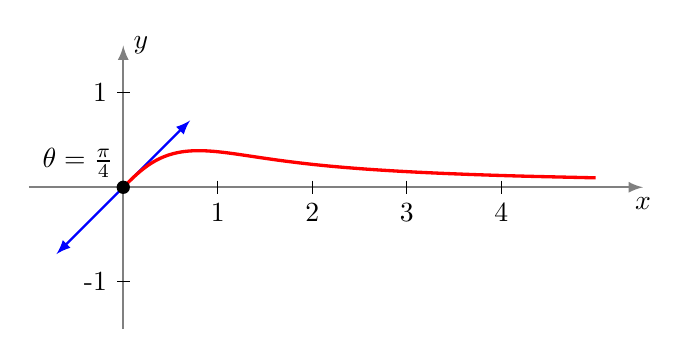
\begin{tikzpicture}[scale=1.2]

% Axes
     \draw[->,>=latex,thick, gray] (-1,0)--(5.5,0) node[below,black] {$x$};
     \draw[->,>=latex,thick, gray] (0,-1.5)--(0,1.5) node[right,black] {$y$};  

 % Ticks
        \foreach \x in {1,...,4}
                \draw (\x,2pt) -- (\x,-2pt)
                        node[anchor=north] {\x};
        \foreach \x in {1}
                \draw (2pt,\x) -- (-2pt,\x)
                        node[anchor=east] {\x};
        \foreach \x in {-1}
                \draw (2pt,\x) -- (-2pt,\x)
                        node[anchor=east] {\x};

  \draw[->,>=latex,thick, blue] (0,0)--+(45:1);
  \draw[->,>=latex,thick, blue] (0,0)--+(45:-1);

% Courbe

\draw [very thick, color=red, domain=0.02:pi/4, samples=100, smooth]
  plot (xy polar cs:angle=\x r, radius={1/sqrt(tan(2*\x r)});
% \draw [very thick, color=gray, domain=3.162:3.92, samples=100, smooth]
%   plot (xy polar cs:angle=\x r, radius={1/sqrt(tan(2*\x r)});

   \fill (0:0) circle (2pt) node[above left] {$\theta=\frac\pi4$};

\end{tikzpicture}  
\end{center}
L'expression $r(\theta)=\frac{\sin^2\theta}{\cos\theta}$ est bien définie sur $\mathcal{D}=]-\frac\pi2,\frac\pi2[$.
\begin{itemize}
Réduction du domaine d'étude\\
Comme $r$ est paire, il suffit en fait de faire l'étude pour les $\theta>0$, donc 
sur $[0;\frac{\pi}{2}[$, 
puis de compléter  par réflexion d'axe $(Ox)$, en effet
$M(-\theta) = s_{(Ox)}(M(\theta))$.

On se restreint donc dans la suite à $\theta\in[0,\frac{\pi}{2}[$, puis on obtient la courbe 
complète par réflexion d'axe $(Ox)$.
Passages par l'origine\\
La courbe passe par l'origine si $r$ s'annule: pour $\theta\in[0,\frac{\pi}{2}[$,
$$r(\theta)=0\Longleftrightarrow\theta=0$$
Variations et signe de la fonction $r$\\
La fonction $r$ est strictement croissante sur $]0,\frac{\pi}{2}[$, 
strictement positive sur $\left]0,\frac{\pi}{2}\right]$ et s'annule en $0$:
$$\begin{array}{c|lcr}
\theta&0&\ &\frac{\pi}{2}\\\hline
\ & &\ & +\infty\\
r&\ &\nearrow &\ \\
 &0 &\ & \\
\end{array}$$
Ainsi la courbe tourne en s'éloignant de l'origine.
Tangente à l'origine\\
La courbe passe par l'origine en $\theta=0$. Par conséquent, la tangente en $O=M\left(0\right)$ est la droite passant par $O$ et d'angle polaire $0$, c'est-à-dire l'axe $(Ox)$.
\'Etude des branches infinies\\
Lorsque $\theta$ tend vers $\frac{\pi}{2}$, $r(\theta)$ tend vers $+\infty$: il y a donc une branche infinie. Pour étudier sa nature, passons en coordonnées cartésiennes:
\begin{eqnarray*}
x(\theta)&=&\sin^2\theta\xrightarrow[\theta\to \frac{\pi}{2}^-]{}1\\
y(\theta)&=&\frac{\sin^3\theta}{\cos\theta}\xrightarrow[\theta\to \frac{\pi}{2}^-]{}+\infty
\end{eqnarray*}
Ainsi la droite d'équation $x=1$ est asymptote verticale. 
\end{itemize}


\begin{center}
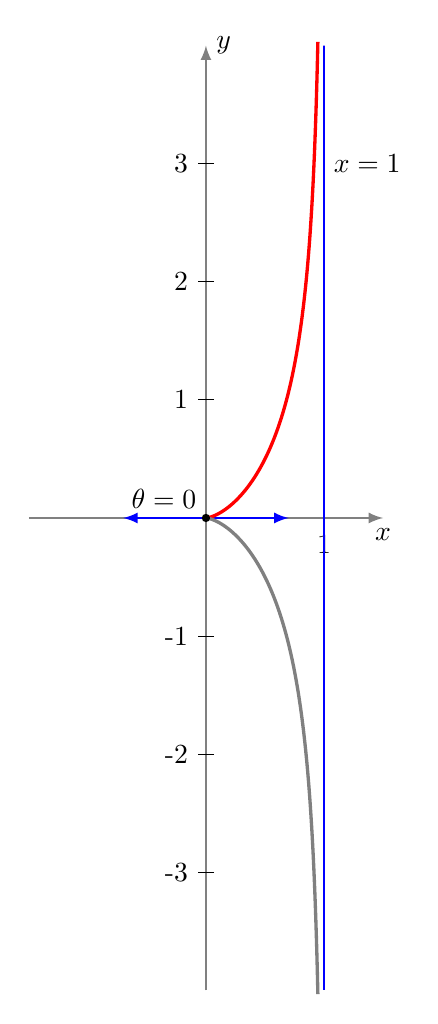
\begin{tikzpicture}[scale=1.5]

% Axes
     \draw[->,>=latex,thick, gray] (-1.5,0)--(1.5,0) node[below,black] {$x$};
     \draw[->,>=latex,thick, gray] (0,-4)--(0,4) node[right,black] {$y$};  

 % Ticks
        \foreach \x in {1,...,1}
                \draw (\x,2pt) -- (\x,-2pt)
                        node[anchor=north] {\x};
        \foreach \x in {1,2,3}
                \draw (2pt,\x) -- (-2pt,\x)
                        node[anchor=east] {\x};
        \foreach \x in {-1,-2,-3}
                \draw (2pt,\x) -- (-2pt,\x)
                        node[anchor=east] {\x};

  \draw[->,>=latex,thick, blue] (0,0)--+(0:0.7);
  \draw[->,>=latex,thick, blue] (0,0)--+(0:-0.7);

% Courbe

\draw [very thick, color=red, domain=0:1.34, samples=100, smooth]
  plot (xy polar cs:angle=\x r, radius={sin(\x r)^2/(cos(\x r)});

\draw [very thick, color=gray, domain=0:-1.34, samples=100, smooth]
  plot (xy polar cs:angle=\x r, radius={sin(\x r)^2/(cos(\x r)});


   \fill (0,0) circle (1pt) node[above left] {$\theta=0$};

  \draw[thick, blue] (1,0)--+(0,4)--+(0,-4);
  \node[right] at (1,3) {$x=1$};
\end{tikzpicture}  
\end{center}
L'expression $r(\theta)=\sqrt{\cos(2\theta)}$ est bien définie si $\cos(2\theta)$ est positif, \textsl{i.e.} sur $\mathcal{D}=\bigcup_{k\in\Z}[-\frac{\pi}{4}+k\pi;\frac{\pi}{4}+k\pi]$.
\begin{itemize}
Réduction du domaine d'étude\\
La fonction $r$ est $\pi$-périodique: on l'étudie sur un intervalle de longueur $\pi$, par exemple $[-\frac{\pi}{2};\frac{\pi}{2}]\cap\mathcal{D}=[-\frac{\pi}{4};\frac{\pi}{4}]$, puis on complète par rotation d'angle $\pi$. De plus $r$ est paire: $\theta\in D\Leftrightarrow-\theta\in D$, et pour $\theta\in D$ on a
$$M(-\theta)=\left[r(-\theta):-\theta\right]=\left[r(\theta):-\theta\right]=s_{(Ox)}(M(\theta))$$
Finalement, on étudie et on construit la portion de courbe correspondant à $\theta\in[0,\frac{\pi}{4}]$, puis on obtient la courbe complète d'abord par réflexion d'axe $(Ox)$, puis par rotation d'angle $\pi$ (symétrie centrale par rapport à l'origine).
Passages par l'origine\\
La courbe passe par l'origine si $r$ s'annule: pour $\theta\in[0,\frac{\pi}{4}]$,
$$r(\theta)=0\Longleftrightarrow\theta=\frac{\pi}{4}$$
Variations et signe de la fonction $r$\\
La fonction $r$ est strictement décroissante sur $[0,\frac{\pi}{4}]$, strictement positive sur $\left]0,\frac{\pi}{4}\right]$ et s'annule en $\frac{\pi}{4}$:
$$\begin{array}{c|lcr}
\theta&0&\ &\frac{\pi}{4}\\\hline
\ &1 &\ & \\
r&\ &\searrow &\ \\
 & &\ &0 \\
\end{array}$$
Ainsi la courbe tourne en se rapprochant de l'origine.
Tangentes\\
La courbe passe par l'origine en $\theta=\frac{\pi}{4}$, et donc la tangente en $M\left(\frac{\pi}{4}\right)$ est la droite passant par $O$ et d'angle polaire $\frac{\pi}{4}$ c'est-à-dire la première bissectrice. 

En $\theta=0$, $r(0)=1$ (et $r'(0)=0$) et la tangente est dirigée par le vecteur
$$\overrightarrow{\frac{\dd M}{\dd \theta}}(0)=r'(0)\vec{u}_0+r(0)\vec{v}_0=\vec{v}_0=\vec{j}$$
et la tangente à la courbe au point $M(0)$ de coordonnées cartésiennes $(1,0)$ est donc verticale.
\end{itemize}

\begin{center}
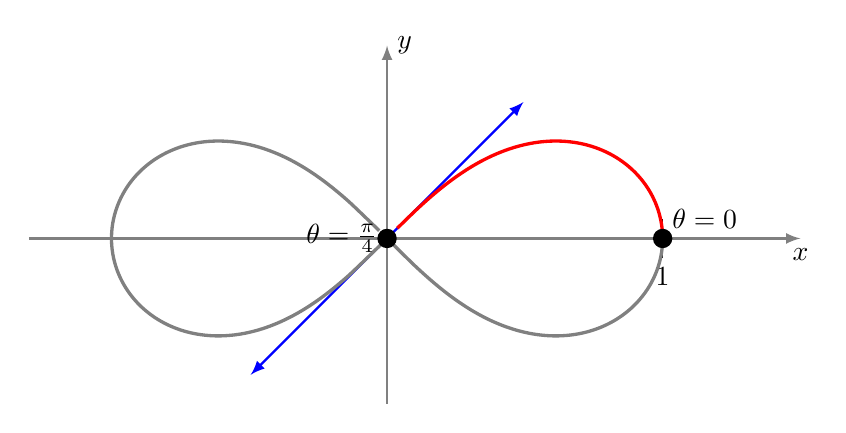
\begin{tikzpicture}[scale=3.5]

% Axes
     \draw[->,>=latex,thick, gray] (-1.3,0)--(1.5,0) node[below,black] {$x$};
     \draw[->,>=latex,thick, gray] (0,-0.6)--(0,0.7) node[right,black] {$y$};  

 % Ticks
        \foreach \x in {1,...,1}
                \draw (\x,2pt) -- (\x,-2pt)
                        node[anchor=north] {\x};
%       \foreach \x in {1}
%               \draw (2pt,\x) -- (-2pt,\x)
%                       node[anchor=east] {\x};
%       \foreach \x in {-1}
%               \draw (2pt,\x) -- (-2pt,\x)
%                       node[anchor=east] {\x};

  \draw[->,>=latex,thick, blue] (0,0)--+(45:0.7);
  \draw[->,>=latex,thick, blue] (0,0)--+(45:-0.7);

% Courbe

\draw [very thick, color=red, domain=0:pi/4, samples=100, smooth]
  plot (xy polar cs:angle=\x r, radius={sqrt(cos(2*\x r)});

\draw [very thick, color=gray, domain=-pi/4:0, samples=100, smooth]
  plot (xy polar cs:angle=\x r, radius={sqrt(cos(2*\x r)});

\draw [very thick, color=gray, domain=2.357:5*pi/4, samples=100, smooth]
  plot (xy polar cs:angle=\x r, radius={sqrt(cos(2*\x r)});


   \fill (0:0) circle (1pt) node[left] {$\theta=\frac\pi4$};
   \fill (1,0) circle (1pt) node[above right] {$\theta=0$};
\end{tikzpicture}  
\end{center}
}
\end{enumerate}
}
